% This LaTeX was auto-generated from MATLAB code.
% To make changes, update the MATLAB code and export to LaTeX again.

\documentclass{article}

\usepackage[utf8]{inputenc}
\usepackage[T1]{fontenc}
\usepackage{lmodern}
\usepackage{graphicx}
\usepackage{color}
\usepackage{hyperref}
\usepackage{amsmath}
\usepackage{amsfonts}
\usepackage{epstopdf}
\usepackage[table]{xcolor}
\usepackage{matlab}

\sloppy
\epstopdfsetup{outdir=./}
\graphicspath{ {./part01a_pzplot_mlx_images/} }

\begin{document}

\matlabtitle{Plotting the poles and zeroes.}


\begin{par}
\begin{flushleft}
The transfer function
\end{flushleft}
\end{par}

\begin{matlaboutput}
G2 =
 
        25
  --------------
  s^2 + 4 s + 25
 
Continuous-time transfer function.
\end{matlaboutput}

\begin{par}
\begin{flushleft}
converts to zero-pole-gain form
\end{flushleft}
\end{par}

\begin{matlaboutput}
G2_zpk =
 
        25
  ---------------
  (s^2 + 4s + 25)
 
Continuous-time zero/pole/gain model.
\end{matlaboutput}

\begin{par}
\begin{flushleft}
We find the zeroes
\end{flushleft}
\end{par}

\begin{matlaboutput}
G2_zero =

  0x1 empty double column vector
\end{matlaboutput}

\begin{par}
\begin{flushleft}
and poles
\end{flushleft}
\end{par}

\begin{matlaboutput}
G2_pole = 2x1 complex    
  -2.0000 + 4.5826i
  -2.0000 - 4.5826i

\end{matlaboutput}

\begin{par}
\begin{flushleft}
Next we plot these as points with the real part as the x-component and the imaginary part as the y-component.
\end{flushleft}
\end{par}

\begin{center}
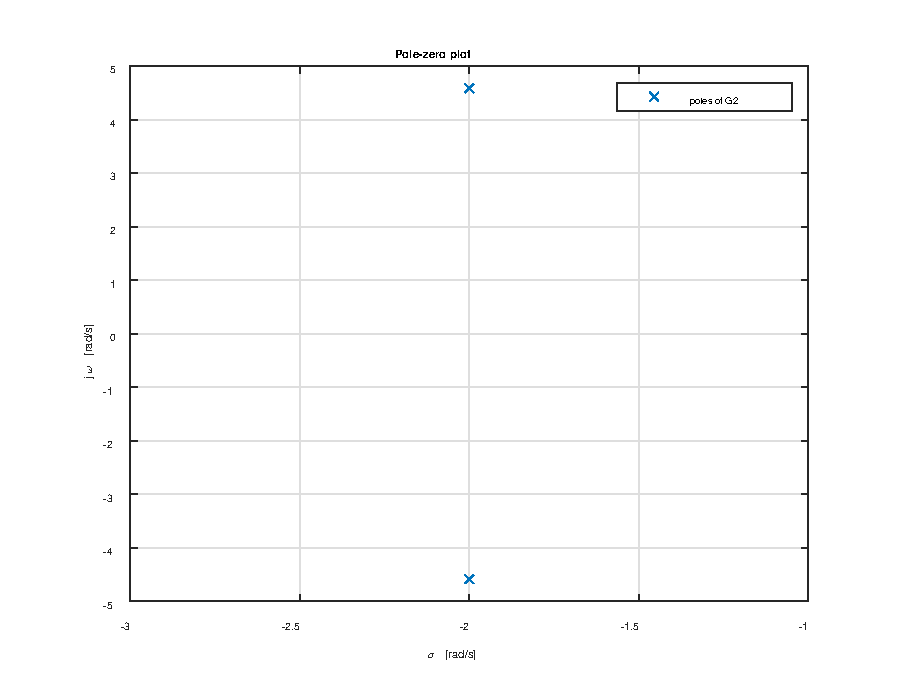
\includegraphics[width=\maxwidth{56.196688409433015em}]{figure_0.eps}
\end{center}
\end{document}
